\chapter{Ekstraksi Fitur Bentuk}
\section{Pendahuluan}
\label{sec:citrabiner}
Fitur bentuk citra diperoleh dengan terlebih dahulu membentuk citra biner, citra yang hanya memiliki dua nilai intensitas piksel, masing-masing \texttt{0} yang mewakili warna hitam dan \texttt{255} yang mewakili warna putih. \textit{Object of interest} akan diberi warna putih, sementara \textit{background} akan diberi warna hitam. Pembentukan citra biner memerlukan proses \textit{thresholding}, proses untuk menentukan titik batas yang dari titik itulah piksel dengan intensitas tertentu diubah menjadi \texttt{0}, sedangkan piksel lain nilai intensitasnya diubah menjadi \texttt{1}. Proses \textit{thresholding} ini mensyaratkan masukan berupa citra dalam skala keabuan.

Pada pustaka \texttt{scikit-image}, proses \textit{thresholding} tersedia melalui beberapa fungsi yang didefinisikan di sub modul \texttt{skimage.filters}. Pustaka \texttt{scikit-image} bahkan menyediakan sebuah fungsi yang dapat digunakan untuk melakukan komparasi visual terhadap hasil \textit{thresholding} menggunakan berbagai metode yang disediakan secara terpisah.

\lstlistingname~\ref{lst:tryAllTh} menunjukkan fungsi komparasi berbagai metode \textit{thresholding} yang disediakan oleh pustaka \texttt{scikit-image}. Pembentukan citra biner dilakukan terhadap citra yang disajikan pada \figurename~\ref{fig:tulips}. Di \lstlistingname~\ref{lst:tryAllTh}, citra dibaca dalam skala keabuan. Sedangkan \figurename~\ref{fig:tulipsGray} menunjukkan hasil citra binernya.

\scriptsize
\lstinputlisting[language=python, numbers=left, numberstyle=\tiny, caption=Melihat kinerja \textit{thresholding} secara visual, showstringspaces=false, label=lst:tryAllTh]{script/tryAllTh.py}
\normalsize

\begin{figure}
  \begin{center}
    \includegraphics[scale=.25]{pics/tulips.png}
    \caption{Citra bunga tulip}
    \label{fig:tulips}
  \end{center}
\end{figure}

\begin{figure}
  \begin{center}
    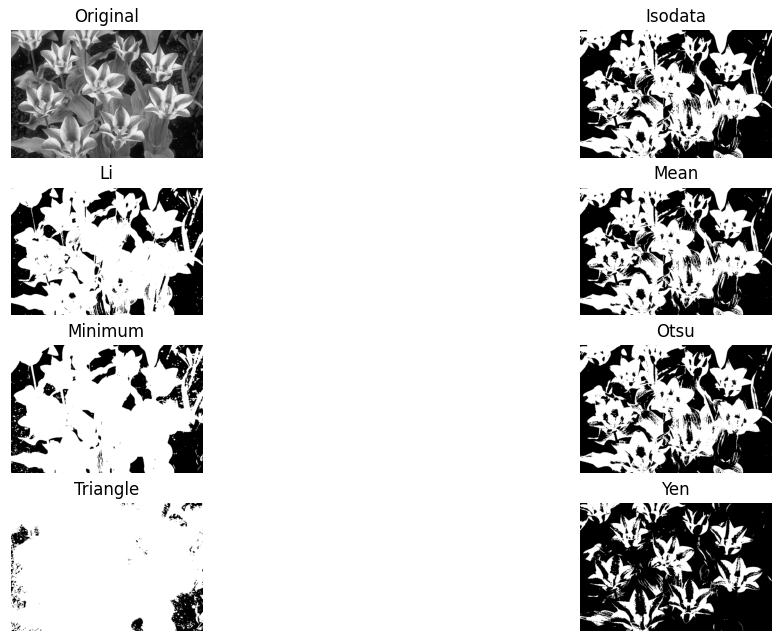
\includegraphics[scale=.65]{pics/tryAllthTulipsGray.png}
    \caption{Citra biner yang dihasilkan dari citra tulips dalam skala keabuan}
    \label{fig:tulipsGray}
  \end{center}
\end{figure}

Seperti telah dijelaskan di sub bab \ref{sec:histogramIntro}, komponen warna merah, hijau dan biru ketika disimpan secara \textit{independent}, akan ditampilkan sebagai citra dalam skala keabuan. Tentunya, nilai \textit{threshold} yang diperoleh dari setiap komponen warna akan berbeda, meski metode \textit{thresholding}nya sama. \figurename~\ref{fig:tryThRed} menunjukkan pembentukan citra biner dari komponen warna merah. Sedangkan \figurename~\ref{fig:tryThGreen} dan \figurename~\ref{fig:tryThBlue} masing-masing menunjukkan proses yang sama berdasarkan komponen warna hijau dan biru. Terlihat bahwa citra biner yang diperoleh berdasarkan komponen warna merah menghasilkan segmentasi yang lebih baik daripada yang diperoleh dari komponen warna hijau dan biru. 

Kekurangan yang masih ada pada citra biner dari komponen warna merah adalah adanya bagian hijau dalam lingkup kelopak bunga. Komponen warna hijau tersebut direpresentasikan sebagai nilai intensitas yang lebih kecil daripada nilai \textit{threshold} ketika direpresentasikan dalam komponen warna merah. Inilah yang menyebabkan kelopak bunga tampak berlubang di bagian tengah. Dari \figurename~\ref{fig:tryThRed}, hanya metode \textit{thresholding} \texttt{Yen} yang mampu membatasi daerah kelopak bunga menjadi satu kesatuan. Kekurangannya adalah, obyek lain di luar kelopak bunga masih dianggap \textit{object of interest}.

Pendekatan ini dapat dilakukan dengan menyisipkan perintah \texttt{img=a[:,:,0]} di antara baris ke-5 dan 6 dari \lstlistingname~\ref{lst:tryAllTh} jika ingin menggunakan komponen warna merah sebagai basis pembentukan citra biner. Sedangkan penyisipan perintah \texttt{img=a[:,:,1]} dan \texttt{img=a[:,:,2]} masing-masing ditujukan untuk menggunakan komponen warna hijau dan biru sebagai basis pembentukan citra biner. Sebagai tambahan, argumen ke-2 pada baris ke-5 dari \lstlistingname~\ref{lst:tryAllTh} ditiadakan. Sedangkan argumen pertama pada baris ke-6 dari \lstlistingname~\ref{lst:tryAllTh} diubah menjadi \texttt{img}, menyesuaikan variabel untuk setiap komponen warna.

\begin{figure}
   \begin{center}
     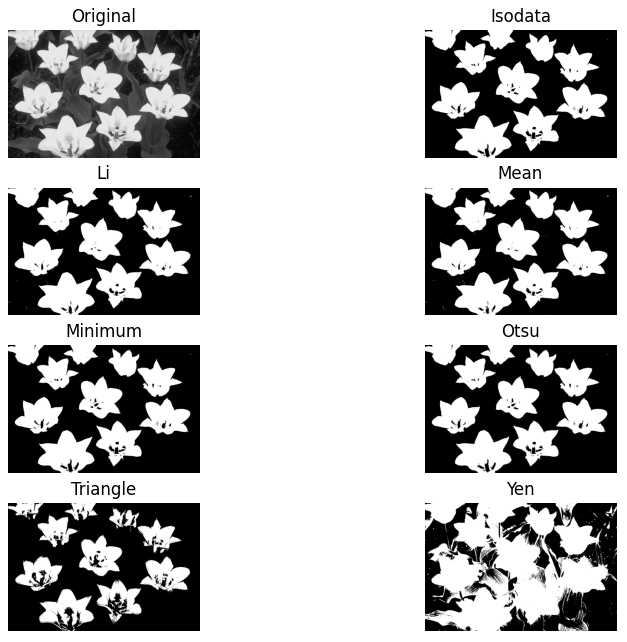
\includegraphics[scale=.65]{pics/tryAllthTulipsRed.png}
     \caption{Citra biner yang dihasilkan dari komponen warna merah dari citra tulips}
     \label{fig:tryThRed}
   \end{center}
 \end{figure} 
 
 \begin{figure}
   \begin{center}
     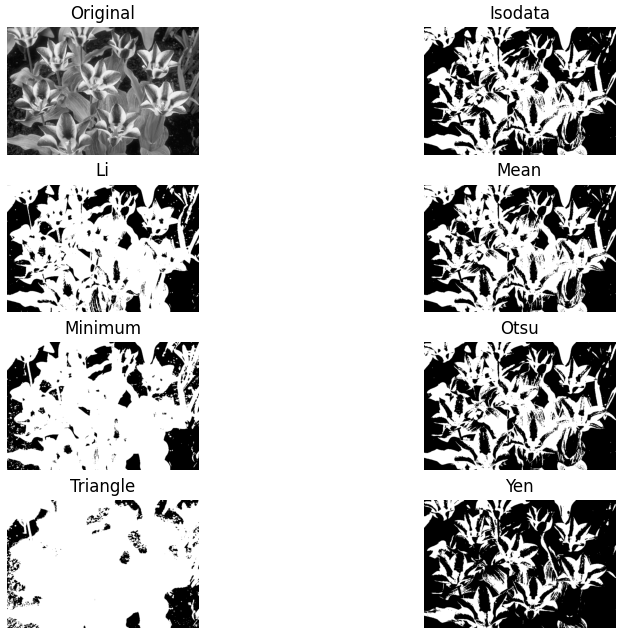
\includegraphics[scale=.65]{pics/tryAllthTulipsGreen.png}
     \caption{Citra biner yang dihasilkan dari komponen warna hijau dari citra tulips}
     \label{fig:tryThGreen}
   \end{center}
 \end{figure}
 
 \begin{figure}
   \begin{center}
     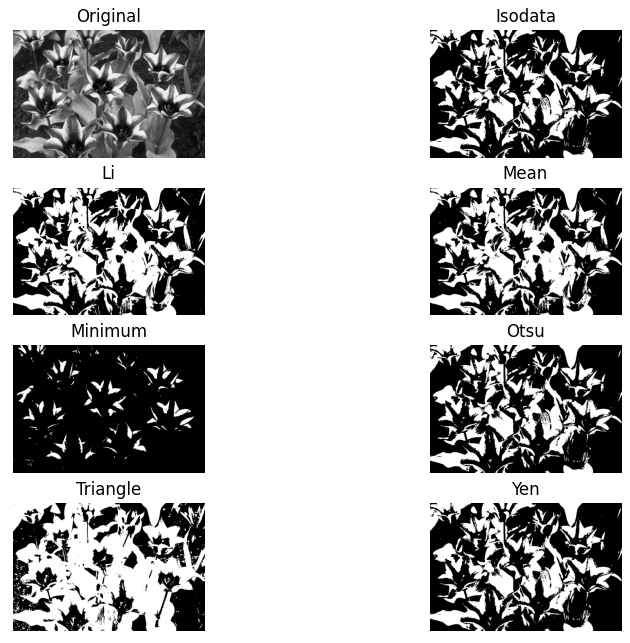
\includegraphics[scale=.65]{pics/tryAllthTulipsBlue.png}
     \caption{Citra biner yang dihasilkan dari komponen warna biru dari citra tulips}
     \label{fig:tryThBlue}
   \end{center}
 \end{figure}
 
 \section{Jumlah obyek pada citra}
Untuk mendapatkan fitur bentuk, obyek harus dapat terpisah secara utuh dari latar (\textit{background}). Pemisahan obyek dari latar ditunjukkan oleh citra biner yang sebelumnya dipelajari di sub bab \ref{sec:citrabiner}. Citra biner sendiri dapat dengan mudah diperoleh ketika obyek dan latar sangat berbeda seperti pada kasus di sub bab \ref{sec:regionprops}. Tetapi, ketika citra yang dihadapi memiliki obyek dan latar yang rumit (\figurename~\ref{fig:tulips}), pembentukan citra biner sangat sulit dilakukan. Untuk alasan inilah, banyak penelitian yang dilakukan terkait segmentasi obyek pada citra \cite{WANG20181}.
 
Salah satu kriteria segmentasi obyek yang baik adalah ditemukannya jumlah obyek yang sama \cite{CREVIER2008143}. Mendeteksi keberadaan obyek secara otomatis dilakukan dengan fungsi blob, yang dalam pustaka \texttt{scikit-image} diterapkan sebagai fungsi \texttt{blob\_dog}, \texttt{blob\_doh} dan \texttt{blob\_log} di bawah sub modul \texttt{skimage.feature}. Basis identifikasi yang digunakan ketiga fungsi tersebut adalah pola hubungan intensitas piksel di mana sebuah obyek didefinisikan sebagai daerah dengan intensitas tinggi yang dikelilingi daerah dengan intensitas rendah atau sebaliknya. 

Untuk mengidentifikasi kondisi tersebut, ketiga fungsi membutuhkan sejumlah argumen yang hampir sama. Dan argumen yang paling penting adalah \texttt{min\_sigma} dan \texttt{max\_sigma}. Seperti telah dijelaskan di sub bab \ref{sec:freqDenoizing}, perubahan intensitas citra dapat dinyatakan dalam bentuk frekuensi. Frekuensi tinggi merupakan representasi dari perubahan intensitas citra yang signifikan, sedangkan frekuensi rendah merupakan representasi dari intensitas citra yang cenderung stabil (tetap). Di sisi lain, frekuensi berbanding terbalik dengan $\sigma$. Semakin besar frekuensi, semakin kecil $\sigma$. Demikian sebaliknya. Argumen \texttt{min\_sigma} dan \texttt{max\_sigma} digunakan untuk mendeteksi daerah pada citra yang memiliki rentang frekuensi tersebut karena di situlah diduga terdapat batas obyek, daerah yang sebelumnya memiliki perubahan intensitas yang cepat kemudian melambat dan stabil. 

Berikut contoh penggunaan ketiga fungsi tersebut.

\subsection{\textit{Difference of Gaussian}}
 
 
 \section{Fitur bentuk}
 \label{sec:regionprops}
Berikut adalah fitur bentuk yang dapat diperoleh menggunakan pustaka \texttt{scikit-image}, yang dalam hal ini didefinisikan sebagai fungsi \texttt{regionprops} di dalam sub modul \texttt{measure}. Sebagai obyek kajian, \lstlistingname~\ref{lst:fiturFlavia} digunakan untuk mengambil sejumlah fitur bentuk dari fungsi \texttt{regionprops}, khususnya yang bernilai tunggal. Fitur titk pusat (\textit{centroid}) dari \textit{object of interest} juga akan diekstrak dengan memisahkannya menjadi titik pusat \texttt{X} dan \texttt{Y}. Citra yang akan diambil fitur bentuknya adalah citra daun flavia\footnote{\url{http://flavia.sourceforge.net/}}. Penggunaan citra tersebut disebabkan karena hanya ada obyek daun yang terdapat di setiap citra, sehingga tidak diperlukan lagi tahapan segmentasi. \lstlistingname~\ref{lst:fiturFlavia} juga akan membentuk berkas fitur dengan format \texttt{csv} yang siap dilatih dengan algoritma pelatihan tertentu. Fitur bentuk yang akan diekstrak adalah yang didefinisikan oleh Putzu \cite{PUTZU2014179}.

\lstlistingname~\ref{lst:fiturFlavia} terdiri dari dua komponen utama, masing-masing komponen data \textit{lookup} untuk melihat kelas daun yang juga didefinisikan di laman \textit{repository} flavia. Data \textit{lookup} tersebut dijalankan oleh fungsi \texttt{leavesClass} di baris ke-7 yang menerima ID daun yang juga menjadi nama berkas daun yang bersangkutan. Sedangkan komponen berikutnya adalah ekstraksi fitur dan menuliskannya pada berkas fitur yang diberi nama \texttt{feature.csv}. 

\scriptsize
\lstinputlisting[language=python, numbers=left, numberstyle=\tiny, caption=Pembentukan berkas fitur bentuk dari obyek daun Flavia, showstringspaces=false, label=lst:fiturFlavia]{script/regionpropsAll.py}
\normalsize
